\documentclass{article}
\usepackage[utf8]{inputenc}
\usepackage{multicol}
\usepackage[margin={1.25in,1.25in}]{geometry}
\usepackage{titlesec}
\usepackage{titling}
\usepackage{graphicx}
\usepackage[
    backend=biber,
    style=ieee,
    url=false, 
    doi=false,
    eprint=false
]{biblatex}

\usepackage{parskip}

\title{Final Paper}
\author{Ryan Bruno}
\date{\today}

\addbibresource{bib.bib}

\renewcommand{\maketitle}{
    \begin{center}
        \Huge\textbf{\thetitle}
    \end{center}
    \begin{multicols}{2}
        \begin{flushright}
        By: \theauthor
        \end{flushright}

        \columnbreak
        
        \thedate
    \end{multicols}
}

\begin{document}

\maketitle

\begin{multicols}{2}
\begin{refsection}
%\large

\section*{Abstract}

While the cost of digital storage is at an all-time low data accumulation of unnecessary replication metadata comes at a cost. Conflict-free Replicated Data Types are being used to ensure consistency throughout a distributed system but many proposed solutions do not take into account memory consumption and simply allow for unbounded metadata growth. In this paper, we explore two methods of memory reduction in the form of garbage collection.

\section*{Introduction}

In order to maintain data availability, large-scale systems not only have to keep multiple copies of their data on different nodes but they must also allow nodes to make changes or make decisions based on that data without a quorum of nodes being available. This leads to variance among nodes and in the past developers would have to create their own algorithms to handle data invariance manually \cite{kleppmann_conflict-free_2017}. It was clear that a solution needed to be described in a way that developers who are already familiar with normal data types could understand and use. This leads us to an abstraction that builds upon traditional data types but provides certain guarantees to avoid distributed conflicts called Conflict-Free Replicated Data Types (CRDTs). CRDTs provide the guarantee that when two or more nodes merge they will always end in the same state. It is also guaranteed that synchronous writes will both be kept in a merge; meaning no write ever gets lost \cite{shapiro_comprehensive_2011}.

\section*{Literature Review}

\subsection*{System Description}

To start we will first describe the types of systems that are applicable for the use of CRDTs. The primary two targets are large-scale systems and limited connectivity devices. Large-scale systems are those deployed by large web-services or companies that must serve many clients spread all around the globe \cite{tao_merging_2015} \cite{balegas_making_2016}. The amount of nodes in those systems grows and shrinks rapidly therefore we assume the amount of total amount of nodes in the system at any point in time is not known, nor can we rely on any type of quorum to be present to make decisions. The second type of system includes limited connectivity devices. This could be a mobile device for which it's user can make changes to data locally but, with an unreliable network connection, the application is not expected to be able to sync with a server in order to make those changes \cite{perkins_simba:_2015}. Some other system requirements are listed below:

Node: We assume all nodes can connect at some point in the future and are synchronous; so they can communicate, merge, and change data in distinctly different periods of time.

Data: A piece of data, unless otherwise specified, is assumed to be immutable and has no relationship to other data. We leave up to implementation how to generate a view of the data as it should not affect the merging algorithm.

Merge: The CRDTs described here are state-based CRDTs as opposed to operation-based CRDTs. During the merge of a state-based CRDT, we assume one node sends its entire data set to another where it is merged with the target's data set \cite{shapiro_comprehensive_2011}.


\subsection*{Grow-Only Set}

One of the most simple CRDTs is a set that only has an add operation. In math a set has two operations add() and remove(). If we allow both these two operations a problem arises when merging two nodes as we cannot determine which node has the most up-to-date data. For example, if node A deletes an element then, to stay consistent in a merge, node B should delete that element as well. However, what should happen if before the merge node B removed the element then added it back? With that in mind, the easiest solution is to not allow the remove operation \cite{shapiro_comprehensive_2011}. It may sound useless but grow-only sets are deployed in a lot of places from logs to your bank account; which is nothing more than a set of transactions that cannot be removed (in the event of a chargeback a new reversal transaction is added). Being one of the most simple CRDTs it is also the most simple to prove. The merging semantics of a Grow-Only set is a simple union which is a commutative operation; meaning both nodes will end in the same state. Lastly, due to the way we chose to represent data synchronous adds are not a problem.

\subsection*{Two-Phase Set}

Building off the previous problem, conflicts arise when a node deletes an item but an algorithm cannot determine if the item should be deleted or, in the case of another node adding the item back after it was deleted, it should stay. This leads us to the next solution which is to allow adds and removes but once an item is removed it cannot be added back \cite{shapiro_comprehensive_2011}. This is called a Two-Phase Set or 2P-Set and is accomplished using tombstones. When a node deletes an item it sets a special marker on that item telling all other nodes to delete that item. No node should re-add an item as the algorithm will always favor removes.


\subsection*{OR-Set}

The idea of an OR-Set builds on the previous logic asking ``can we get around the re-add restriction by adding a random id to each added item?" An OR-set automatically adds an id to every item that is added to the set and this alone lifts any restrictions on the add or remove operations \cite{shapiro_comprehensive_2011}. Now we have a CRDT that has no restrictions on the add or remove function; similar to a math set. We can guarantee that all sets will merge without any conflicts as long as the ids are generated randomly. An application can now also update data in the set by simply removing an item, changing it, then adding it back. Traditional developers may ask the question ``What happens when two nodes change a value at the same time?" The answer is that both values will be left in the set and while this may be a problem for some applications for others this is a feature. The possible projects below showcase some weird examples of how we can change our view on application data from this equals that to something more CRDT friendly.

\subsection*{Relationships}

In order to allow for the easy transition from relational database schema, we can provide a mechanism for handling relationships in a distributed environment. We can provide such this mechanism with two changes \cite{balegas_making_2016}. To exemplify these changes lets begin with a one-to-many relationship between managers and employees. If a node would like to add a new employee under a manager the node would add to the set both the employee, the manager, and the relationship between them. This is the first change and provides the foreign key integrity constraints that are familiar in most relational databases as a synchronous delete of the manager would be canceled out by the addition of the manager back into the set. This type of merge is called ``last writer wins" and may not be ideal for some situations for example if we really want to delete a manager. In order to do this, we create a new set used by the merging algorithm. In our example, if we would like to delete manager ``m" we tell the merge algorithm to drop every item matching ``m" and relationship R(m,*). This would not allow the manager nor any relationship with the manager to return.

\subsection*{Garbage-Collection}

OR-Sets are great in many ways but one of its drawbacks is the accumulation of tombstones. The only job of a tombstone is to ensure the deletion of an item in other nodes and once every node has seen the tombstone it can be safely be deleted from every node \cite{bauwens_memory_2019}. There are two solutions to this problem that can both be used simultaneously. Both solutions require us to force our system to have a known finite number of nodes and must ensure local operation ordering. The first solution piggyback on the idea that tombstones may be deleted when they are no longer needed and operation ordering. A single node will ignore tombstones originating from another if the latest item it has received from the originating node is grater then the item in question. This prevents incorrect reappearance of items and allows nodes to remove a tombstone once it has received it from the nodes where it has originated. The second solution trades collection rate for network overhead. If an originating node broadcasts an operation it must hear back from each node for the operation to be casually stable. This may take a while as nodes could be buffering responses. Eager collection speeds this process up by requiring an acknowledgment then broadcasting stability status of an operation so then every node knows that metadata before a certain timestamp is no longer necessary. The rate at which a node does this is a point of configuration.

\subsection*{Stream Parsing}

There are some situations where it is better to process data as a stream moving through the system than to store the individual updates. An example of this would be ``likes" on a social media post. It does not make sense to store every like in a set if we only want a number of how many people like the post. If there is only one globally writable integer associated with that post we run into the same data race problem that occurs in multithreaded programs. The CRDT solution is to create a set containing a different counter for each node \cite{navalho_incremental_2013}. Since every node is synchronous it can safely increment its own counter but no others. When we want to compute the final number we sum every node's counter. In the case of a very large system, a small set of nodes can be picked as ``allowed to increment the counter" nodes and all other requests can be forwarded to them. As a more complex example, we can use this to solve a top-N problem \cite{navalho_incremental_2013}. If we would like to get the top 20 posts then each post would get a counter that functions the exact same as before. However, now each node has to sort each counter and display the top-N posts.

\subsection*{Resettable Counter}

Building off the last solution of a CRDT counter, we can add a reset function. Each node is still only allowed to write to one item in the list but now associated with the counter is a ``freshness" value \cite{baquero_problem_2016}. When a reset is required a node sets its value to zero and increments its ``freshness" value. When merging with another node if any freshness values are incremented then that node must reset its own value. 


\section*{Example Applications}

Listed below are two example applications that show the power of CRDTs in action. The examples should show how to view program data is a more CRDT friendly way. Not all the implementation details are listed however there should be enough to understand the big picture.

\subsection*{Distributed Text Editing}

One of the most classic examples of CRDTs in use is with a distributed text editor. In order to achieve this a position value can be given to each item of the set \cite{kleppmann_conflict-free_2017}. If we give an absolute position to a character then a merge with another node may leave newly added items in a location that does not make sense anymore. The solution is to use an OR-Set and add the id of the previous item to each item. This creates a sort of linked list including items who have been replaced with a tombstone. When two items point to the same parent we know there has been a conflict and implementations will usually display one entire string first then the other. One node may add a word after another that has been deleted synchronously. In this case, once the two merge the first word will be replaced with a tombstone and not displayed to the user but will still be present and can be referenced by the new word; holding its position correctly.

\section*{Primary Objective}

To measure the memory reduction of using garbage collection in combination with an OR-Set while keeping the properties of a Conflict-free Replicated Data Type. Limited to 1.5 person weeks over 12 weeks.

\section*{Solution Description}

The two areas that need to be described are the software that implements the OR-Set algorithm with garbage collection and the environment that allows the objective the be met. The node software will communicate over TCP/IP and will be written in C or C++. The underlying data set will be one compatible with the C++ standard template library's unordered\_map. This data type is the same as a hash map and will allow us to create a relationship between id $\rightarrow$ data, change the mapping from id $\rightarrow$ data to id $\rightarrow$ tombstone, and remove an id completely. A merging algorithm then needs to be built into this data type along with both garbage collection algorithms. The environment is the domain in which where nodes operate and communicate. There will be one Administrator node that holds no data and is not considered apart of the system to garbage collection algorithms. The job of the administrator node is to provide a way for the experiment administrator to induce artificial network delays and packet losses. This allows us to see how the algorithm works under heavy network delay despite them being located on the same LAN or same physical machine.


\section*{Hypothesis}

While the data size of a nodes not using garbage collection will grow linearly with the amount of operations; using garbage collection will eventually be bounded if the dataset is bounded.

\subsection*{Goals Tree}


%Goal G1 => To measure and compare the memory efficiency of using garbage collection.

%Goal G1.1 => To obtain the total memory consumption of a system not using garbage collection.

%Goal G1.2 => To assess the efficiency of the casually stable and eager garbage collection methods.

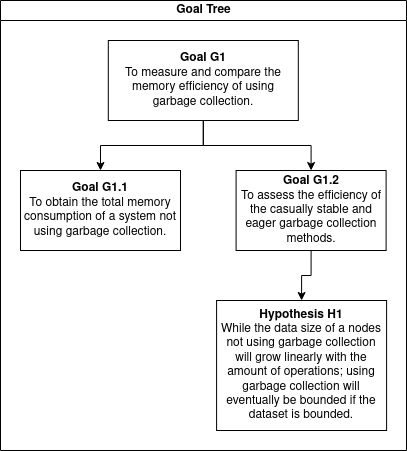
\includegraphics[width=\columnwidth]{goal_tree}

\section*{Experiment Design}

There are many variables that may come into play in this experiment. As such we have decided to hold some variables constant, allow for some to vary but keep these in mind when analyzing the results, and vary some intentionally to test how it affects the results. Developers of large scale system software do not design their software to fail but, with a large enough system, administrators can account for a regular node failure due to hardware or software malfunctions. This is why, as a governing proposition, we set the amount of initial nodes at five, add two nodes every minute, and force a node to fail every minute. To ensure the accumulation of garbage we will also keep consistent the ratio of adds to remove operations. Once a starting data set is in place a node will, when given the ability to issue an operation due to random chance, always add after a remove and remove after an add. The frequency at which this happens will be intentionally changed along with the eager collection rate. These two variables will be tested while keeping in to account nodes system size variation at constant intervals to compare the growth rate of total memory consumption.

\section*{Conclusion}

This paper has served to introduce topics from the concept of Conflict-free Replicated Data Types with a focus on memory efficiency. This along with a description of a solution lays a framework for a concrete experiment to confirm for deny our hypothesis and accomplish the aforementioned goals.

\printbibliography[title=References]
\end{refsection}

\end{multicols}


\end{document}
